% Main report of Stage 1: the three implementations (Java, Python, C++) and their comparison.
% Build from docs/report/:
%   uv run --with matplotlib python charts.py     (figures/*.pdf, from the three languages' committed CSVs)
%   pdflatex report.tex && pdflatex report.tex     (twice, for the table of contents)
% The finished report is copied to docs/Stage1_Report.pdf.
\documentclass[11pt,a4paper]{article}

\usepackage[utf8]{inputenc}
\usepackage[T1]{fontenc}
\usepackage{lmodern}
\usepackage{microtype}
\usepackage[margin=2.4cm,headheight=14pt]{geometry}
\usepackage{graphicx}
\usepackage{booktabs}
\usepackage{tabularx}
\usepackage{array}
\usepackage{enumitem}
\usepackage{float}
\usepackage{xcolor}
\usepackage{amssymb}
\usepackage{listings}
\usepackage{tikz}
\usetikzlibrary{positioning,arrows.meta,calc}
\usepackage{fancyhdr}
\usepackage{titlesec}
\usepackage[hidelinks]{hyperref}

\definecolor{accent}{HTML}{2a78d6}
\definecolor{ink}{HTML}{0b0b0b}
\definecolor{muted}{HTML}{52514e}
\definecolor{codebg}{HTML}{f6f6f4}
\definecolor{rule}{HTML}{d8d7d2}
\definecolor{notebg}{HTML}{eef4fc}

\hypersetup{colorlinks=true,linkcolor=accent,urlcolor=accent,citecolor=accent}

\titleformat{\section}{\Large\bfseries\color{ink}}{\thesection.}{0.6em}{}
\titleformat{\subsection}{\large\bfseries\color{ink}}{\thesubsection}{0.6em}{}
\titleformat{\subsubsection}{\normalsize\bfseries\color{ink}}{\thesubsubsection}{0.6em}{}
\titlespacing*{\section}{0pt}{1.6em}{0.7em}
\titlespacing*{\subsection}{0pt}{1.2em}{0.5em}

\pagestyle{fancy}
\fancyhf{}
\fancyhead[L]{\small\color{muted}Stage 1 $\cdot$ Data layer $\cdot$ Main report}
\fancyhead[R]{\small\color{muted}Big Data $\cdot$ ULPGC}
\fancyfoot[C]{\small\thepage}
\renewcommand{\headrulewidth}{0.4pt}

\setlist{itemsep=2pt,topsep=4pt}
\setlength{\parskip}{0.45em}
\setlength{\parindent}{0pt}
\setlength{\emergencystretch}{3em}
\renewcommand{\arraystretch}{1.25}

\lstdefinestyle{shell}{
  language={}, basicstyle=\ttfamily\footnotesize, backgroundcolor=\color{codebg}, frame=single,
  rulecolor=\color{rule}, framesep=4pt, xleftmargin=6pt, xrightmargin=6pt,
  breaklines=true, columns=fullflexible, keepspaces=true, showstringspaces=false,
  aboveskip=8pt, belowskip=8pt}
\lstset{style=shell}

\newcolumntype{Y}{>{\raggedright\arraybackslash}X}
\newcolumntype{L}[1]{>{\raggedright\arraybackslash}p{#1}}
\newcommand{\code}[1]{\texttt{#1}}
\newcommand{\us}{\,$\mu$s}
\newcommand{\win}{\bfseries}   % the fastest language in a table row
\newenvironment{note}{\par\smallskip\noindent
\begin{tikzpicture}\node[fill=notebg,draw=accent!40,rounded corners=2pt,inner sep=7pt,text width=\dimexpr\linewidth-14pt\relax]\bgroup\small}{\egroup;\end{tikzpicture}\par\smallskip}

\begin{document}

% ---------------------------------------------------------------- title page
\hypersetup{pageanchor=false}
\begin{titlepage}
\thispagestyle{empty}
\vspace*{2.5cm}
{\color{accent}\rule{\linewidth}{1.2pt}}\\[0.8cm]
{\Huge\bfseries Search Engine Project\par}
\vspace{0.4cm}
{\LARGE Stage 1: Building the Data Layer\par}
\vspace{0.6cm}
{\Large\color{muted} Main report --- three implementations compared: Java, Python and C++\par}
\vspace{0.6cm}
{\color{accent}\rule{\linewidth}{1.2pt}}
\vspace{2cm}

\begin{tabular}{@{}>{\bfseries}L{3.4cm}L{10.5cm}@{}}
Course & Big Data $\cdot$ Grado en Ciencia e Ingeniería de Datos $\cdot$ Universidad de Las Palmas de Gran Canaria \\
Academic year & 2026/2027 \\
Group name & BigData-Ulpgc \\
Members & Daniel Rodríguez Alonso --- 79072763M --- Java implementation \\
 & Daniel Perdomo Medina --- 54173402F --- Python implementation \\
 & Carlos Falcón Brito --- 54149163X --- C++ implementation \\
Repository & \url{https://github.com/BigData-Ulpgc/stage_1} \\
Module reports & \code{java/stage1/docs/Stage1\_Java\_Report.pdf}, \code{python/stage\_1/docs/Stage1\_Python\_Report.pdf}, \code{cpp/docs/Stage1\_Cpp\_Report.pdf} \\
Date & 4 October 2026 \\
\end{tabular}

\vfill
\begin{note}
\textbf{How to read this report.} Sections~\ref{sec:intro}--\ref{sec:impl} describe the common data
layer and how each language implements it, and Section~\ref{sec:decisions} justifies the structures
selected. Section~\ref{sec:bench} presents the benchmarks of the datalake, the metadata and the
inverted index, and compares the execution times of the three implementations on the same data. Section~\ref{sec:choice} uses that
comparison to choose the language that best fits the project. Each module's own report gives the
class-by-class detail that is only summarised here.
\end{note}
\end{titlepage}
\hypersetup{pageanchor=true}

% ---------------------------------------------------------------- abstract + toc
\section*{Abstract}
Stage~1 of the group's search engine over Project Gutenberg builds the \emph{data layer}: a pipeline
that downloads books, splits them into header and body, stores them in a datalake, extracts their
metadata into SQLite and builds an inverted index that answers Boolean AND queries, with a control
layer that lets an interrupted run resume without losing or repeating books. The group implemented
the same data layer three times, in \textbf{Java}, \textbf{Python} and \textbf{C++}, against one
written contract (\code{shared/SPEC.md}). The three implementations produce identical outputs: the
same 128,980,349 bytes in the datalake and the same 129,356 terms and 1,581,064 postings in the index
of the 200 books.

All three run the same 12 benchmark experiments with the same methodology, so their execution times
can be compared. The index experiments of the three languages, and every Java and Python experiment,
ran on the same Linux machine. On that common ground, \textbf{C++ is the fastest} wherever work is done
in the program itself (AND queries 3.2 times faster than Java and 21 times faster than Python on the
\code{monolithic} index), \textbf{Java stays within 1.1--3.2 times of C++} on queries and is the
fastest at updating the \code{monolithic} index, and \textbf{Python is 2--21 times slower} wherever an
interpreted loop runs per term or per query, while matching the others when the work happens in the
operating system, SQLite, JSON or MongoDB. The three languages agree on the structures to use
(\code{book} datalake, \code{monolithic} index, SQLite with indexes). Weighing performance together
with development effort, deployment, safety and the ecosystem for the next stages, the report
recommends \textbf{Java} as the language of the project, with C++ reserved for a latency-critical
query service and Python for analysis and tooling.

\tableofcontents
\newpage

% ================================================================ 1
\section{Introduction and objectives}\label{sec:intro}

\subsection{Goal of Stage 1}
The course project builds a search engine over the books of Project Gutenberg in several stages.
Stage~1 leaves ranking and user interfaces for later and builds the data underneath: the books must be
downloaded and kept, their metadata extracted and their words indexed, \emph{correctly}, in a way
that \emph{survives interruptions}, and \emph{measurably}, so that different ways of storing the same
data can be compared with numbers.

The assignment asks for:
\begin{itemize}
  \item a \textbf{datalake} for the raw books, and \textbf{datamarts} with structured data ready to
        query: the book metadata and an inverted index;
  \item a minimal \textbf{control layer} that never duplicates or loses work;
  \item \textbf{benchmarks} of alternative datalake and inverted-index structures,
  \item implemented in \textbf{at least three programming languages} over the same data.
\end{itemize}

\subsection{How the group organised the work}
Each member implemented the complete data layer in one language (Table~\ref{tab:team}). So that
three programs written by three people could be compared, the group first wrote a common contract,
\code{shared/SPEC.md}, which fixes everything that must not differ between languages
(Table~\ref{tab:spec}), and a shared set of inputs: the 200 book ids, the stopwords, the query
workload and a 15-book sample dataset for offline tests. Everything outside the contract (the
internal design, libraries, tests) was each member's choice, and that freedom is part of what the
comparison measures.

\begin{table}[H]
\centering\small
\begin{tabularx}{\linewidth}{@{}L{3.6cm} L{2.0cm} Y@{}}
\toprule
Member & Language & Folder and report \\
\midrule
Daniel Rodríguez Alonso & Java 17 & \code{java/stage1/} $\cdot$ \code{docs/Stage1\_Java\_Report.pdf} \\
Daniel Perdomo Medina & Python 3 & \code{python/stage\_1/} $\cdot$ \code{docs/Stage1\_Python\_Report.pdf} \\
Carlos Falcón Brito & C++20 & \code{cpp/} $\cdot$ \code{docs/Stage1\_Cpp\_Report.pdf} \\
\bottomrule
\end{tabularx}
\caption{The group and the three implementations.}
\label{tab:team}
\end{table}

\begin{table}[H]
\centering\small
\begin{tabularx}{\linewidth}{@{}L{1.3cm} L{2.9cm} Y@{}}
\toprule
SPEC & Topic & What it fixes for every language \\
\midrule
\S1 & Inputs & \code{book\_ids.txt} (200 ids, in order), \code{queries.txt}, \code{stopwords.txt}; blank and \code{\#} lines ignored. \\
\S2 & Download and split & The Gutenberg URL; the \code{*** START/END OF THE/THIS PROJECT GUTENBERG EBOOK} markers (a book without both is discarded); header and body trimmed; \code{\textbackslash r\textbackslash n} $\rightarrow$ \code{\textbackslash n}. \\
\S3 & Datalake layouts & \code{time}: \code{YYYYMMDD/HH/<ID>.body.txt}; \code{book}: \code{<ID>/body.txt}; \code{range}: \code{01000-01999/<ID>.body.txt}. \\
\S4 & Metadata & Four multi-line regexes (title, author, release date, language); SQLite table \code{books} with indexes on \code{author} and \code{title}. \\
\S5 & Tokenizer & ASCII only: A--Z lowered, a--z and 0--9 form tokens, anything else separates; tokens of 2+ characters; stopwords removed; a book contributes its \emph{set} of terms. \\
\S6 & Index structures & \code{monolithic} (one JSON file), \code{hierarchical} (\code{<LETTER>/<term>.txt}), \code{mongo} (one document per term); posting lists sorted, without duplicates. \\
\S7 & Queries & Same tokenizer; AND = intersection; ids in ascending order. \\
\S8 & Control layer & \code{downloaded\_books.txt} and \code{indexed\_books.txt}; an id is appended only after its step succeeded. \\
\S9--10 & Benchmarks & The 12 experiments; CSV \code{language,experiment,structure,} \code{dataset\_size,repetition,metric,value,unit}; 2 warm-ups + 5 measured runs; no network inside a measurement; the reference term counts. \\
\bottomrule
\end{tabularx}
\caption{The common contract, \code{shared/SPEC.md}, in short.}
\label{tab:spec}
\end{table}

\subsection{What the group delivers}
\begin{table}[H]
\centering\small
\begin{tabularx}{\linewidth}{@{}Y c c c@{}}
\toprule
 & Java & Python & C++ \\
\midrule
Complete pipeline: crawler, datalake, metadata, index, AND search, control & \checkmark & \checkmark & \checkmark \\
Three datalake layouts and three persistent index structures & \checkmark & \checkmark & \checkmark \\
Offline mode over \code{sample\_dataset/raw/} & \checkmark & \checkmark & \checkmark \\
The 12 SPEC experiments, results committed in the common CSV format & \checkmark & \checkmark & \checkmark \\
Automated tests (all passing) & 357 & 39 & 232 \\
\bottomrule
\end{tabularx}
\caption{Status of the three implementations on 4 October 2026.}
\end{table}

% ================================================================ 2
\section{System architecture}\label{sec:arch}

\subsection{Pipeline overview}
The data layer separates unstructured content from structured, queryable data:
\begin{itemize}
  \item The \textbf{datalake} keeps every downloaded book as two plain-text files, its header and its
        body (the licence footer is dropped). It is the single source from which every datamart can
        be rebuilt.
  \item The \textbf{datamarts} hold what later stages query: the \textbf{metadata} of each book
        (title, author, language, release date and the paths of its files) in SQLite, and the
        \textbf{inverted index}, which maps each term to the sorted ids of the books that contain it.
  \item The \textbf{control layer} records which books are downloaded and which are indexed, and
        decides the next operation.
  \item A \textbf{query module} answers AND queries over the inverted index, so the pipeline can be
        checked end to end (\code{search whale island} returns books 76, 84 and 2701 in the three
        languages).
\end{itemize}
Figure~\ref{fig:arch} follows one book through the data layer. The three implementations share
these components and this data flow; they differ in how each component is written.

\begin{figure}[H]
\centering
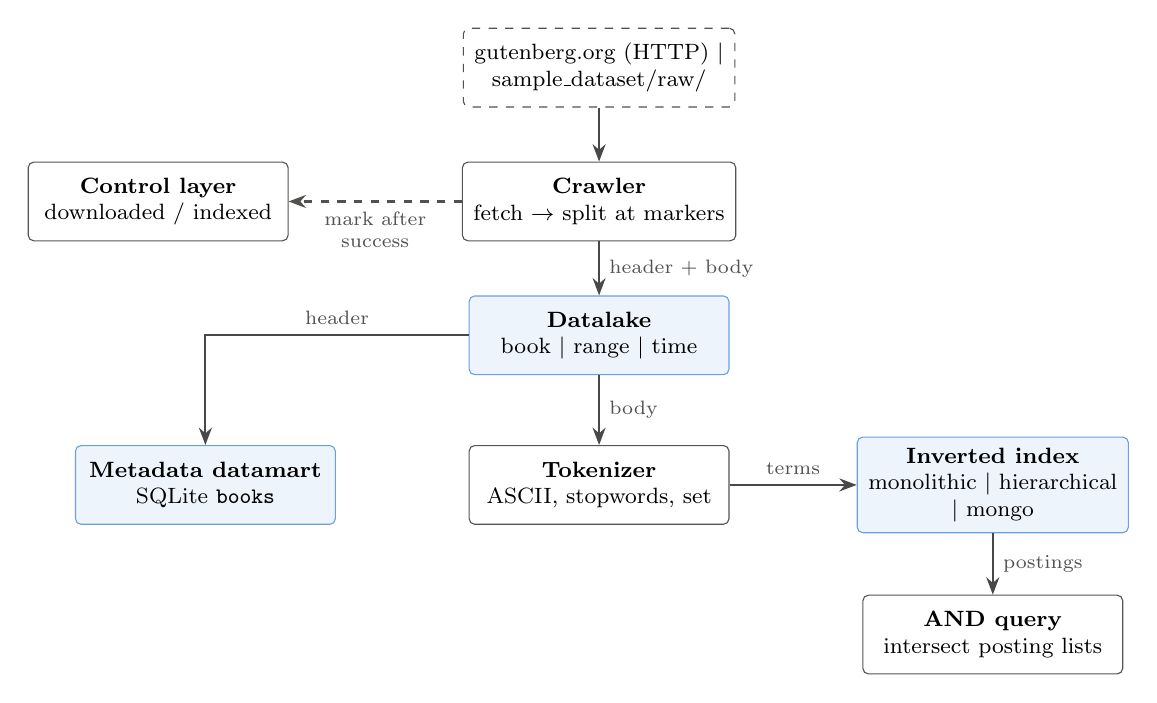
\begin{tikzpicture}[
  font=\footnotesize,
  box/.style={draw=ink!70,rounded corners=2pt,align=center,minimum height=1.0cm,inner sep=4pt,fill=white,minimum width=3.3cm},
  store/.style={box,fill=notebg,draw=accent!70},
  ext/.style={box,dashed,draw=muted},
  arr/.style={-{Stealth[length=2.2mm]},thick,draw=ink!75},
  lbl/.style={font=\scriptsize,color=muted}]
  \node[ext] (src) at (0,0) {gutenberg.org (HTTP) $|$\\sample\_dataset/raw/};
  \node[box] (crawl) at (0,-1.7) {\textbf{Crawler}\\fetch $\rightarrow$ split at markers};
  \node[store] (lake) at (0,-3.4) {\textbf{Datalake}\\book $|$ range $|$ time};
  \node[store] (meta) at (-5.0,-5.3) {\textbf{Metadata datamart}\\SQLite \code{books}};
  \node[box] (tok) at (0,-5.3) {\textbf{Tokenizer}\\ASCII, stopwords, set};
  \node[store] (idx) at (5.0,-5.3) {\textbf{Inverted index}\\monolithic $|$ hierarchical\\$|$ mongo};
  \node[box] (q) at (5.0,-7.2) {\textbf{AND query}\\intersect posting lists};
  \node[box] (ctrl) at (-5.6,-1.7) {\textbf{Control layer}\\downloaded / indexed};
  \draw[arr] (src) -- (crawl);
  \draw[arr] (crawl) -- node[right,lbl]{header + body} (lake);
  \draw[arr] (lake) -| node[pos=0.25,above,lbl]{header} (meta);
  \draw[arr] (lake) -- node[right,lbl]{body} (tok);
  \draw[arr] (tok) -- node[above,lbl]{terms} (idx);
  \draw[arr] (idx) -- node[right,lbl]{postings} (q);
  \draw[arr,dashed,draw=muted] (crawl) -- node[below,lbl,align=center]{mark after\\success} (ctrl);
\end{tikzpicture}
\caption{The data layer of Stage~1, common to the three implementations.}
\label{fig:arch}
\end{figure}

\subsection{The structures under comparison}
\begin{table}[H]
\centering\small
\begin{tabularx}{\linewidth}{@{}L{2.7cm} L{4.7cm} Y@{}}
\toprule
Structure & Layout & Expected trade-off \\
\midrule
\multicolumn{3}{@{}l}{\textit{Datalake}} \\
\code{book} & \code{<ID>/header.txt}, \code{body.txt} & Path computed from the id; one root entry per book. \\
\code{range} & \code{01000-01999/<ID>.body.txt} & Path computed from the id; at most 2,000 files per folder. \\
\code{time} & \code{YYYYMMDD/HH/<ID>.body.txt} & Arrival order and small folders; the path cannot be computed from the id. \\
\midrule
\multicolumn{3}{@{}l}{\textit{Inverted index}} \\
\code{monolithic} & One JSON \code{\{"term":[ids]\}} & Everything in memory: fast queries; each update rewrites the whole file. \\
\code{hierarchical} & \code{inverted\_index/} \code{<L>/<term>.txt} & Updates touch only a book's terms; one small file per term. \\
\code{mongo} & Collection \code{inverted\_index}, unique index on \code{term} & Data in a server: cheap updates, shared by processes; a round trip per term. \\
\midrule
\multicolumn{3}{@{}l}{\textit{Metadata}} \\
\code{sqlite} & Table \code{books} + indexes on \code{author}, \code{title} & Fast lookups by author or title, slower inserts. \\
\code{sqlite\_no\_index} & The same table without those indexes & The baseline: full scans. \\
\bottomrule
\end{tabularx}
\caption{The structures that the benchmarks compare.}
\end{table}

\subsection{Control layer}\label{sec:control}
The control layer follows the decision process of the assignment, with two control files in
\code{data/control/}: \code{downloaded\_books.txt} and \code{indexed\_books.txt}, one id per line.
\begin{enumerate}
  \item \textbf{Index first.} If a book is downloaded but not indexed, it is indexed: its header is
        parsed into the metadata datamart and its body is tokenized and added to the inverted index.
  \item \textbf{Otherwise download.} The next id of \code{shared/book\_ids.txt} that is not in
        \code{downloaded\_books.txt} is downloaded, split and stored in the datalake, so a book is
        never downloaded twice. Instead of the random ids of the assignment's example, the group uses
        a fixed list of 200 ids, so the three languages process exactly the same books and every id
        is known to have both markers.
  \item \textbf{Update the state.} The id is appended to the matching control file only after the
        operation has been written to disk.
\end{enumerate}
Java and C++ implement this loop literally: each \code{pipeline} step performs one download or one
indexing, indexing first. Python processes each book completely in one step (download, then index
into the three structures) and marks it after each phase; the effect on the control files is the
same. In Stage~1 the control layer is sequential, as the assignment requires; parallel downloaders
and indexers are left for later stages.

\subsection{Reliability rules shared by the three implementations}
\begin{itemize}
  \item \textbf{Mark after doing.} An id is appended to a control file only after its step was
        written. The worst case after a crash is repeating one step, never losing a book.
  \item \textbf{Idempotent operations.} Saving a book, upserting metadata, adding a document to an
        index (sets, \code{\$addToSet}) can be repeated safely after a failure.
  \item \textbf{A half-written control line is ignored.} If a process dies in the middle of an
        append, the fragment is not glued to the next id (``13'' + ``84'' $\neq$ ``1384'').
  \item \textbf{An ASCII-only tokenizer.} Unicode-aware lowercasing behaves differently in each
        language; walking the bytes against fixed ranges makes the three indexes identical.
\end{itemize}

% ================================================================ 3
\section{How each language implements the data layer}\label{sec:impl}

\subsection{Java}
\textbf{Stack.} Java 17 (tested on OpenJDK 21) built with Maven; \code{java.net.http.HttpClient} for
downloads, \code{sqlite-jdbc} for SQLite, Jackson for JSON, the synchronous MongoDB driver, and
JUnit~5. About 4,800 lines in 44 classes and interfaces, plus 5,200 lines of tests.

\textbf{Design.} The implementation is object-oriented and organised around \textbf{interfaces}:
\code{BookSource}, \code{Datalake}, \code{MetadataRepository} and \code{InvertedIndex}, each with
several implementations. Every class receives its collaborators in the constructor, two factories
map configuration names to classes, and a single assembly class, \code{SearchEngine}, connects the
whole system, so the command line and the tests share exactly the same wiring.
\begin{itemize}
  \item \code{AbstractFileDatalake} is a template method: the three layouts only decide
        \emph{where} a book goes; the base class writes header then body atomically (temporary file
        plus \code{ATOMIC\_MOVE}) and defines what counts as a complete book.
  \item \code{MonolithicJsonIndex} keeps a \code{TreeMap<String, TreeSet<Integer>>} and rewrites the
        JSON when dirty; \code{HierarchicalFolderIndex} rewrites only changed term files;
        \code{MongoInvertedIndex} sends one unordered \code{bulkWrite} of upserts with \code{\$addToSet}.
  \item \code{PipelineController.step()} performs at most one operation, indexing first, then
        downloading; \code{ControlFiles} appends only after success.
  \item The active datalake and index are chosen in \code{config.properties} or with \code{-D}
        options; \code{AppConfig} is the only class that builds paths, and fails at start-up on an
        unknown key or structure.
\end{itemize}

\textbf{Testing.} 357 tests at four levels: unit tests; \emph{contract tests} that run the same
cases against every implementation of \code{Datalake} (36) and \code{InvertedIndex} (33);
integration tests with real SQLite and MongoDB; and end-to-end tests that run the whole program
without network, kill it, reopen it, and check that nothing is downloaded twice.
\code{SampleDatasetTest} checks the split byte by byte against \code{sample\_dataset/book/}.

\textbf{Benchmarks.} Timed with \code{System.nanoTime}; memory read from the JVM heap after
requesting a garbage collection. The two warm-ups also warm up the JIT compiler.

\subsection{Python}
\textbf{Stack.} Python 3.10+ (results with 3.12), \code{requests} and \code{pymongo}; everything else
comes from the standard library (\code{sqlite3}, \code{json}, \code{pathlib}, \code{tracemalloc}).
About 2,900 lines in 26 modules, the shortest of the three, plus 39 \code{pytest} tests.

\textbf{Design.} A modular design with abstract base classes (\code{abc.ABC}) for \code{Datalake}
and \code{InvertedIndex}, frozen dataclasses with \code{\_\_slots\_\_} for the records, and plain
functions for the stateless steps (\code{split\_header\_body}, \code{parse\_metadata},
\code{tokenize}, \code{search}).
\begin{itemize}
  \item \textbf{The pipeline writes every structure at once}: each book goes to the three datalakes
        and the three indexes in the same pass, and all of them are flushed before the book is
        marked as indexed. One run fills everything the benchmarks need, and the structures can never
        drift apart; the price is six writes per book.
  \item Atomic writes with a \code{.tmp} file and \code{os.replace}, in a single helper shared by the
        three layouts.
  \item \code{JavaRandom} and \code{java\_shuffle} port \code{java.util.Random}, so the random lookup
        order and metadata queries are exactly Java's.
  \item A command line (\code{argparse}) with \code{pipeline}, \code{search} and \code{status}.
\end{itemize}

\textbf{Testing.} 39 unit tests, plus checks that run on the real data: every index benchmark calls
\code{verify()} against an in-memory reference index, and \code{verify\_results} checks the committed
CSVs against the exact values of SPEC section 10. Its output was checked byte for byte against
Java's on the 200 books.

\textbf{Benchmarks.} Timed with \code{time.perf\_counter\_ns}; memory measured with
\code{tracemalloc} (objects allocated through Python's allocator). A first run on Windows~11 was many
times slower, because NTFS and the antivirus slowed down the 129,000 small files of the
hierarchical index, so the official results were taken on Linux.

\subsection{C++}
\textbf{Stack.} C++20 with CMake presets and Ninja (\code{make} and \code{make test} as shortcuts);
SQLite3, libcurl and mongo-cxx-driver from the system; nlohmann/json and GoogleTest downloaded by
CMake. About 5,200 lines in 97 header and source files, plus 3,500 lines of tests (232 tests).

\textbf{Design.} The logic lives in a static library, \code{stage1\_core}, and the executable only
parses arguments and dispatches. The code favours \textbf{free functions for decisions}
(\code{split\_book}, \code{extract\_metadata}, \code{tokenize}, \code{query\_and},
\code{next\_control\_action}), which are tested without disk or network, and small interfaces for
what has side effects (\code{Datalake}, \code{IndexWriter}, \code{BookSource}, \code{HttpClient},
\code{Clock}).
\begin{itemize}
  \item \textbf{RAII} owns every resource: the \code{sqlite3*} handle, prepared statements, the curl
        handle, temporary folders in the tests. \code{std::optional} marks expected absence (no
        markers, no book) and exceptions are kept for I/O errors.
  \item The index is an in-memory \code{std::unordered\_map<std::string, std::set<int>>}, rebuilt
        at start-up; an \code{IndexWriter} persists it: \code{write} for the whole index,
        \code{update\_terms} for the terms of one new book. MongoDB updates go in one unordered bulk
        write, as in Java.
  \item The \code{time} datalake remembers the paths it wrote, so its \code{locate} is a map lookup
        (Section~\ref{sec:times-datalake} explains why this matters in the comparison).
  \item \code{JavaRandom}, a 48-bit linear congruential generator with Java's published algorithm,
        replaces \code{<random>}, whose output differs between libc++ and libstdc++.
\end{itemize}

\textbf{Testing.} 232 GoogleTest tests with fake HTTP clients and clocks; the 11 that need MongoDB
are skipped without a server. A development log (\code{cpp/docs/DEVLOG.md}, 72 entries) records each
decision together with its measurements.

\textbf{Benchmarks.} Timed with \code{std::chrono::steady\_clock}; memory read from the allocator
(\code{mallinfo2} on Linux, \code{malloc\_zone\_statistics} on macOS).

\subsection{The three implementations side by side}
\begin{table}[H]
\centering\small
\begin{tabularx}{\linewidth}{@{}L{3.2cm} Y Y Y@{}}
\toprule
 & Java & Python & C++ \\
\midrule
Paradigm & Object-oriented, interfaces, factories & Modules, ABCs, functions & Free functions + small interfaces, RAII \\
Production code & $\sim$4,800 lines, 44 classes & $\sim$2,900 lines, 26 modules & $\sim$5,200 lines, 97 files \\
Tests & 357 (JUnit 5) & 39 (pytest) + run-time checks & 232 (GoogleTest) \\
External libraries & sqlite-jdbc, Jackson, Mongo driver & requests, pymongo & SQLite3, libcurl, mongo-cxx-driver, nlohmann/json \\
Build and install & Maven downloads everything & \code{pip install} & Compiler, CMake, Ninja; native libraries installed by hand \\
Structures in the pipeline & One of each, by configuration & All of them in the same run & One of each, by configuration \\
In-memory index & \code{TreeMap} of \code{TreeSet<Integer>} & \code{dict} of \code{set} & \code{unordered\_map} of \code{std::set<int>} \\
Atomic file writes & Yes (temp + atomic move) & Yes (temp + \code{os.replace}) & No (relies on the control layer) \\
Memory metric & JVM heap after GC & \code{tracemalloc} & Allocator statistics \\
\bottomrule
\end{tabularx}
\caption{The three implementations compared by construction.}
\label{tab:sidebyside}
\end{table}

\subsection{Same output in the three languages}
Before comparing speed, the group checked that the three programs compute the same thing. All of
them produce:
\begin{itemize}
  \item the same datalake: 400 files and 128,980,349 bytes for the 200 books, in every layout, and the
        15 sample books byte-identical to \code{sample\_dataset/book/};
  \item the same index: 58,834 / 78,820 / 129,356 terms and 360,970 / 759,087 / 1,581,064
        postings for $N = 50$ / 100 / 200, and a monolithic JSON of exactly 8,893,537 bytes;
  \item the same answer to the sample query ``whale island'': books 76, 84 and 2701.
\end{itemize}
Every difference reported in the following sections is therefore a difference of \emph{speed or
memory}, never of results.

% ================================================================ 4
\section{Design decisions}\label{sec:decisions}
The assignment asks to justify the selected data structures and indexing strategies. Every
structure is implemented in the three languages and benchmarked in Section~\ref{sec:bench}; this
section states the choice and the reasons, which the three implementations reached independently.

\subsection{Datalake: \code{book}}
\begin{itemize}
  \item \textbf{Lookup.} The path of a book is computed from its id, so a lookup is one existence
        check: 2.5--3.3\us{} in C++ and Java, and the fastest layout in Python too. In the
        \code{time} layout the path depends on when the book was downloaded, so Java and Python must
        walk the hour folders (29 and 14 times slower), a cost that grows with every hour of
        ingestion.
  \item \textbf{Ingestion, incremental detection and recovery.} The three layouts write the same bytes
        at about the same speed, all of them detect exactly the 20 new books and recover the 20
        interrupted ones with nothing lost or duplicated; \code{book} is the fastest or within a few
        milliseconds of it in every language.
  \item \textbf{Storage overhead.} 400 files in every layout; \code{book} adds one folder per book
        (200), a 1.5\% block overhead, negligible at this scale.
  \item \textbf{Why not the recommended \code{time} layout.} Its strengths are traceability, small
        folders (20 entries) and the possibility of processing only the most recent folders. In
        Stage~1 the control files already say which books are new, so nothing benefits from that, while
        every lookup by id pays its cost. The layout stays implemented and selectable.
  \item \textbf{When to change.} With tens of thousands of books, \code{book} puts one entry per book
        in a single root folder; \code{range} keeps the direct lookup and bounds every folder.
\end{itemize}

\subsection{Inverted index: \code{monolithic}, with \code{mongo} as the growth path}
\begin{itemize}
  \item \textbf{At the scale of Stage~1} (200 books, 129,356 terms) \code{monolithic} is the fastest to
        build, to query and, in Java and C++, to update, and the smallest on disk (8.9~MB), in the
        three languages.
  \item \textbf{Its limits are structural}: every update rewrites the whole file, and the whole index
        lives in memory (54--147~MB for 200 books depending on the language). Both grow linearly with
        the collection.
  \item \textbf{\code{hierarchical}} updates only the files of a book's terms and uses almost no memory,
        but its 129,356 small files take 530~MB of disk blocks for 7.3~MB of data (73 times).
  \item \textbf{\code{mongo}} keeps the index out of the process, supports concurrent readers and
        writers and updates one document per term. It is the structure to move to when the
        collection outgrows memory or when several processes share the index (Stage~2), at the cost
        of a network round trip per query term.
  \item \textbf{Indexing strategy, common to all structures.} Terms come from the shared ASCII
        tokenizer with stopwords removed; each book contributes its \emph{set} of terms (no
        frequencies, no positions), and posting lists are kept sorted and without duplicates, so an
        AND query is a linear-time intersection that starts from the shortest list.
\end{itemize}

\subsection{Metadata: SQLite with indexes on \code{author} and \code{title}}
SQLite is embedded, needs no server and is part of the standard tooling of the three languages.
With 100,000 rows, the two indexes make lookups by author 160--380 times faster than a full scan and
keep them flat as the table grows, for a slower insertion that only matters during bulk loads. The
comparison with other backends (PostgreSQL, MongoDB), optional in the assignment, was not carried
out; Section~\ref{sec:future} lists it as future work.

\subsection{Shared implementation decisions}
\begin{itemize}
  \item \textbf{A fixed dataset of 200 real books}, listed in \code{shared/book\_ids.txt}, instead of
        random ids: every language processes the same books, and the result can be checked against
        reference counts.
  \item \textbf{Atomic writes} (temporary file plus rename) in Java and Python, and \textbf{marking
        after doing} in the three, so a crash never leaves a half-written book counted as stored.
  \item \textbf{Configuration instead of code changes}: Java and C++ select the datalake and index in
        \code{config.properties}; Python keeps every structure up to date in each run.
  \item \textbf{MongoDB is optional}: the group's server runs from \code{docker-compose.yml}, and the
        three programs skip the \code{mongo} structure with a warning when it is not reachable.
\end{itemize}

\begin{table}[H]
\centering\small
\begin{tabularx}{\linewidth}{@{}L{2.4cm} L{3.0cm} Y@{}}
\toprule
Part & Choice & Because (holds in the three languages) \\
\midrule
Datalake & \code{book} & Fastest lookup that survives a restart, fast change detection and recovery, same bytes as the others; the benchmarks also read it. \code{range} is the alternative for a far larger catalogue. \\
Inverted index & \code{monolithic} & Fastest build, queries and updates at 200 books, smallest on disk. Its update cost and memory grow with the index; beyond a few hundred to a few thousand books, \code{mongo} (or \code{hierarchical}) takes over. \\
Metadata & \code{sqlite} with indexes & Lookups by author and title stay flat as the table grows, for a modest insertion cost. \\
\bottomrule
\end{tabularx}
\caption{Structures selected for the final implementation.}
\label{tab:selected}
\end{table}

% ================================================================ 5
\section{Benchmarks and results}\label{sec:bench}
This section presents the 12 experiments required by the assignment for the datalake, the metadata
and the inverted index, and compares the three languages in each of them.

\subsection{Methodology}\label{sec:method}

\subsubsection{Common rules}
\begin{itemize}
  \item \textbf{2 warm-ups and 5 measured runs} per experiment; this report uses the \textbf{median}
        of the five, which resists isolated pauses (garbage collection, disk flushes).
  \item \textbf{Preparation is not timed}: clearing folders and databases, opening connections and
        tokenizing the books happen before the clock starts.
  \item \textbf{No network inside a measurement}: the real books are read from a \code{book} datalake
        filled once by the pipeline.
  \item \textbf{Same data, same order}: a size $N$ is the $N$ books with the lowest ids; random
        choices (lookup order, metadata queries) come from the same \code{java.util.Random}
        sequence with seed 42 in the three languages; the \code{time} layout uses a simulated clock
        of 10 books per hour.
  \item \textbf{Verification before reporting}: every experiment checks its result (every book
        found, posting lists equal to an in-memory reference, 0 books lost) and stops instead of
        writing numbers if the check fails.
\end{itemize}

\subsubsection{Experiments and data}
\begin{table}[H]
\centering\small
\begin{tabularx}{\linewidth}{@{}L{4.6cm} L{3.1cm} Y@{}}
\toprule
Experiments & Structures & Data \\
\midrule
\code{datalake\_write}, \code{\_lookup}, \code{\_incremental}, \code{\_recovery}, \code{\_storage} & \code{book}, \code{range}, \code{time} & The 200 real books (129.0~MB) \\
\code{index\_build}, \code{\_query}, \code{\_update}, \code{\_memory}, \code{\_disk} & \code{monolithic}, \code{hierarchical}, \code{mongo} & The 50, 100 and 200 real books with the lowest ids \\
\code{metadata\_insert}, \code{\_query} & \code{sqlite}, \code{sqlite\_no\_index} & 1,000 / 10,000 / 100,000 generated rows (each author has 10 books, each title 2) \\
\bottomrule
\end{tabularx}
\caption{The 12 experiments of SPEC sections 9--10.}
\end{table}
The assignment's \emph{download and write throughput} is measured on the write side only:
downloading depends on Project Gutenberg and the network, which would hide any difference between
structures or languages, so the books are downloaded once by the pipeline and the benchmark times
splitting-free storage of the 200 books. Metadata uses generated rows because 200 real books are
too few to show how SQLite scales; the assignment asks for thousands to tens of thousands of rows.

\subsubsection{Environment: what is directly comparable}
\begin{table}[H]
\centering\small
\begin{tabularx}{\linewidth}{@{}L{3.6cm} Y Y Y@{}}
\toprule
Experiments & Java & Python & C++ \\
\midrule
Index (5 experiments) & Linux & Linux & Linux \\
Datalake (5 experiments) & Linux & Linux & \textbf{macOS, Apple Silicon} \\
Metadata (2 experiments) & Linux & Linux & \textbf{macOS, Apple Silicon} \\
\bottomrule
\end{tabularx}
\caption{Where each set of results was measured. ``Linux'' is one machine: Ubuntu 24.04, 12 threads,
15~GB RAM, NVMe SSD, MongoDB 8.2.12 in Docker; OpenJDK 21 and Python 3.12.}
\label{tab:env}
\end{table}

\begin{note}
\textbf{Reading the comparison.} The \textbf{index} experiments of the three languages, and every
Java and Python experiment, ran on the same Linux machine: there, a difference is a difference of
language and implementation. The C++ \textbf{datalake and metadata} results come from a different
machine and operating system (APFS on Apple Silicon), so for those two families a gap with C++ mixes
the language with the hardware; the figures mark those C++ bars with a hatched pattern. Memory is
measured differently in each language (JVM heap, \code{tracemalloc}, allocator statistics), so its
absolute values are only indicative; how it grows with $N$ is comparable.
\end{note}

\subsection{Datalake}\label{sec:times-datalake}\label{sec:times}
\begin{figure}[H]
\centering
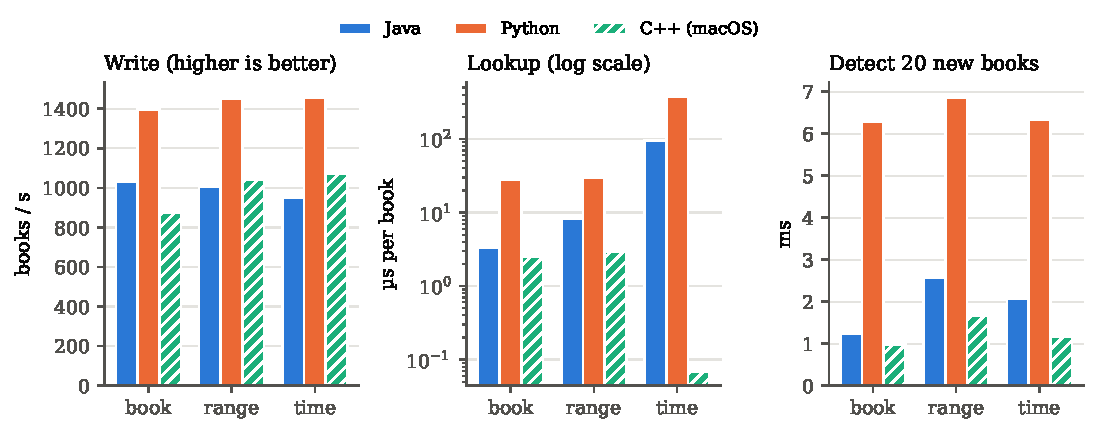
\includegraphics[width=\linewidth]{figures/lang_datalake.pdf}
\caption{Datalake with the 200 real books, median of 5 runs. Hatched: C++, measured on macOS.}
\end{figure}

\begin{table}[H]
\centering\small
\begin{tabular}{@{}llrrr@{}}
\toprule
Metric & Layout & Java & Python & C++\,$^\dagger$ \\
\midrule
Write (books/s) & \code{book} & 1,031 & \win 1,398 & 876 \\
 & \code{range} & 1,006 & \win 1,449 & 1,044 \\
 & \code{time} & 948 & \win 1,458 & 1,071 \\
Lookup (\us/book) & \code{book} & 3.3 & 27.8 & \win 2.5 \\
 & \code{range} & 8.3 & 30.0 & \win 2.9 \\
 & \code{time} & 94.5 & 377.9 & \win 0.07\,$^\ddagger$ \\
Detect 20 new books (ms) & \code{book} & 1.24 & 6.28 & \win 0.98 \\
Recover 20 books (ms) & \code{book} & 23.8 & 22.5 & \win 19.1 \\
\bottomrule
\end{tabular}
\caption{Datalake timings, 200 books. $^\dagger$~measured on macOS. $^\ddagger$~an in-memory map of
the paths written by the process, not a walk of the folders. Bold: the fastest
language. All three recover the 20 damaged books with 0 lost and 0 duplicated, and store the same
bytes (400 files, 129.0~MB).}
\end{table}

\begin{itemize}
  \item \textbf{Writing is bound by the file system, not the language.} The three languages write the
        same 129~MB in 400 files at 880--1,460 books/s, and the layouts differ by about 20\% at most.
        Python is even the fastest: \code{write\_text} hands the whole buffer to the operating system
        in one call, so the interpreter does very little per book.
  \item \textbf{Lookups show the cost of the language around each system call.} A \code{book} or
        \code{range} lookup is one path computation and one existence check. C++ and Java need
        2.5--8\us{}; Python needs about 28\us, because building \code{Path} objects and calling the
        file system from interpreted code costs 8 times more than in Java on the same machine.
  \item \textbf{The \code{time} layout is a design, not a language, result.} Java and Python walk the
        hour folders, newest first, and are 29 and 14 times slower than their own \code{book}
        lookup. C++ remembers the paths it has written, which is fast but does not survive a restart,
        so its 0.07\us{} is not comparable with the other two.
  \item \textbf{Detecting new books} (listing the folders) is again 5 times slower in Python than in
        Java, while \textbf{recovery}, dominated by rewriting 20 books, is equal within 25\% in the three.
\end{itemize}

\begin{table}[H]
\centering\small
\begin{tabular}{@{}lrrrrr@{}}
\toprule
Layout & Files & Folders & Fullest folder & Data (MB) & Allocated (MB) \\
\midrule
\code{book} & 400 & 200 & 200 & 129.0 & 130.9 \\
\code{range} & 400 & 47 & 220 & 129.0 & 130.3 \\
\code{time} & 400 & 21 & 20 & 129.0 & 130.2 \\
\bottomrule
\end{tabular}
\caption{Storage overhead of the datalake, 200 books: identical in the three languages. Besides these
files, every layout uses the same two control files.}
\label{tab:storage}
\end{table}

\textbf{Storage overhead} (Table~\ref{tab:storage}) does not depend on the language: the three write
the same files. It shows the structural trade-off of each layout: \code{time} bounds every folder by
the ingestion rate (20 entries), \code{book} puts one folder per book in the root, and \code{range}
does not spread these ids well, because 110 of the 200 are below 1,000 and share one folder.

\subsection{Inverted index}
This is the family where the comparison is cleanest (same machine for the three languages) and
where most of the program's own work happens.

\begin{figure}[H]
\centering
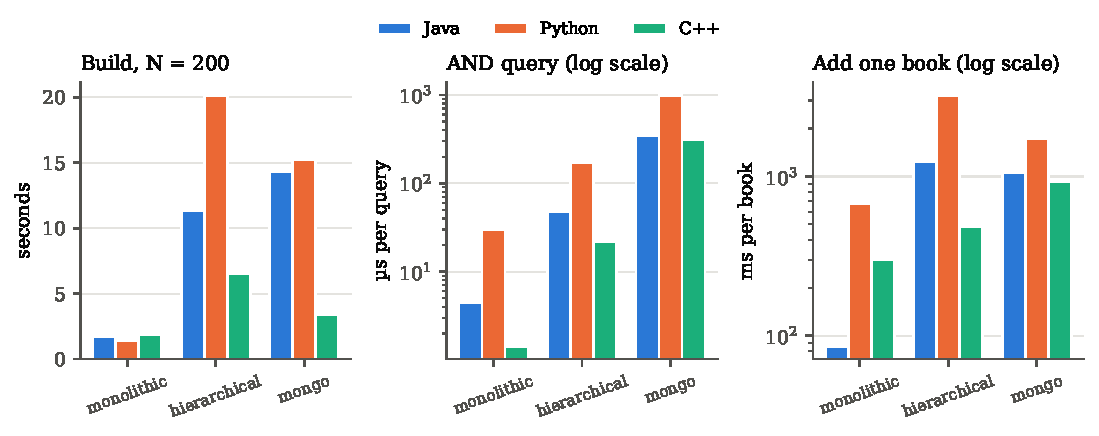
\includegraphics[width=\linewidth]{figures/lang_index.pdf}
\caption{Inverted index with $N = 200$ books, median of 5 runs, same Linux machine for the three languages.}
\end{figure}

\begin{table}[H]
\centering\small
\begin{tabular}{@{}llrrr@{}}
\toprule
Metric ($N = 200$) & Structure & Java & Python & C++ \\
\midrule
Build (s) & \code{monolithic} & 1.69 & \win 1.40 & 1.85 \\
 & \code{hierarchical} & 11.34 & 20.10 & \win 6.55 \\
 & \code{mongo} & 14.29 & 15.23 & \win 3.36 \\
AND query (\us) & \code{monolithic} & 4.5 & 29.6 & \win 1.4 \\
 & \code{hierarchical} & 48.3 & 171.1 & \win 22.0 \\
 & \code{mongo} & 344.8 & 987.7 & \win 314.6 \\
Add one book (ms) & \code{monolithic} & \win 85.4 & 674.0 & 300.0 \\
 & \code{hierarchical} & 1,239 & 3,230 & \win 482 \\
 & \code{mongo} & 1,053 & 1,723 & \win 922 \\
\bottomrule
\end{tabular}
\caption{Inverted index, $N = 200$: 129,356 terms and 1,581,064 postings in every case.}
\label{tab:index}
\end{table}

\subsubsection{Queries: the clearest language effect}
An AND query tokenizes a few words, fetches their posting lists and intersects them. On the
\code{monolithic} index everything is in memory, so the time is pure program execution: C++ answers in
1.4\us, Java in 4.5\us{} (3.2 times) and Python in 29.6\us{} (21 times). Python sorts each posting
list out of a \code{set} and intersects it in an interpreted loop; Java iterates boxed
\code{Integer}s from a \code{TreeSet}; C++ walks contiguous integers.

When the query has to leave the process, the language matters less: on \code{hierarchical} (one file
read per term) the spread shrinks to 2.2 times for Java and 7.8 times for Python, and on \code{mongo}
(one round trip to the server per term) Java is only 10\% slower than C++. The slower the storage,
the smaller the share of the time that the language controls.

\subsubsection{Build and update: language and design mixed}
\begin{itemize}
  \item \textbf{\code{monolithic} build}: the three are within 33\% of each other, and Python is the
        fastest, because filling dictionaries and \code{json.dumps} run in C inside the interpreter.
  \item \textbf{\code{hierarchical} build} creates 129,356 files: C++ needs 6.5~s, Java 11.3~s (1.7
        times) and Python 20.1~s (3.1 times), the overhead of each language per file operation.
  \item \textbf{\code{mongo} build} is 4.3 times faster in C++ for a design reason: it fills an empty
        collection with \code{insert\_many} of whole documents, while Java and Python send one upsert
        with \code{\$addToSet} per term. When the three use the same upsert (the update experiment),
        C++ and Java are within 15\%.
  \item \textbf{\code{monolithic} update} rewrites the whole 8.9~MB JSON after each book. Here
        \textbf{Java is the fastest} (85~ms), ahead of C++ (300~ms) and Python (674~ms): Jackson
        serialises the sorted map directly, the C++ writer goes through nlohmann/json, and Python
        sorts the ids of all 129,356 terms before every write. With the \code{monolithic} build, it is
        one of the two index experiments where C++ is not the fastest, and it is the write path of
        the structure the group selected.
\end{itemize}

\subsubsection{Scaling with the size of the collection}
\begin{figure}[H]
\centering
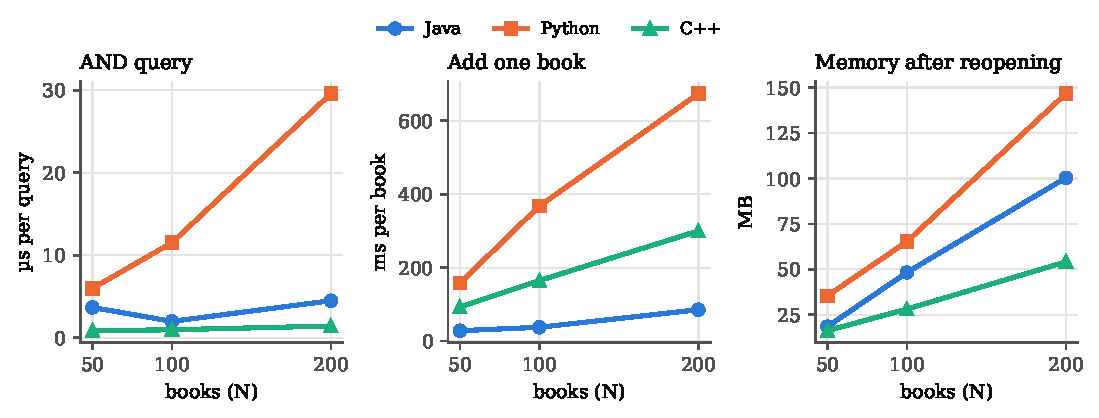
\includegraphics[width=\linewidth]{figures/lang_scaling.pdf}
\caption{The \code{monolithic} index as the collection grows from 50 to 200 books.}
\label{fig:scaling}
\end{figure}

Figure~\ref{fig:scaling} shows how the structure chosen by the three languages scales. The ordering
of the languages does not change with $N$, but the slopes do. Python's update cost grows fastest
(158 $\rightarrow$ 674~ms, 4.3 times for 4 times the books) because its per-flush sort grows with
the index; C++ grows 3.2 times (93 $\rightarrow$ 300~ms) and Java 3.0 times (28 $\rightarrow$
85~ms). Query times stay in the microsecond range in the three languages.

\subsection{Memory and disk}
\begin{table}[H]
\centering\small
\begin{tabular}{@{}lrrr@{}}
\toprule
Memory after reopening the \code{monolithic} index (MB) & Java & Python & C++ \\
\midrule
$N = 50$ & 18.5 & 35.5 & \win 16.3 \\
$N = 100$ & 48.3 & 65.2 & \win 28.1 \\
$N = 200$ & 100.3 & 146.6 & \win 54.1 \\
\bottomrule
\end{tabular}
\caption{Memory held by the open \code{monolithic} index; \code{hierarchical} and \code{mongo} keep
almost nothing ($<$50~KB) in the three languages.}
\end{table}

The same 8.9~MB of JSON occupies 54~MB as C++ \code{std::set<int>}, 100~MB as Java \code{TreeSet}s of
boxed \code{Integer}s (about 63 bytes per posting) and 147~MB as Python \code{set}s of \code{int}
objects. The representation of a posting, not the data, sets the memory cost, and the gap between
languages widens as the index grows, reaching 1 : 1.9 : 2.7 (C++ : Java : Python) at $N = 200$. On disk the three languages write the same bytes
(Table~\ref{tab:disk}).

\begin{table}[H]
\centering\small
\begin{tabular}{@{}lrrrr@{}}
\toprule
Structure ($N = 200$) & Data (MB) & Files & Allocated (MB) & Allocated / data \\
\midrule
\code{monolithic} & 8.9 & 1 & 8.9 & 1.0 \\
\code{hierarchical} & 7.3 & 129,356 & 530.0 & 73.1 \\
\code{mongo} & 13.1--14.1 & --- & --- & --- \\
\bottomrule
\end{tabular}
\caption{Index on disk. The file-based structures are byte-identical in the three languages; for
\code{mongo} the size is the collection plus its index, as reported by the server.}
\label{tab:disk}
\end{table}

Every term file of \code{hierarchical} takes at least one 4~KB block, so 7.3~MB of postings reserve
530~MB: the ``very large number of small files'' that the assignment warns about, measured.

\subsection{Metadata (SQLite)}
\begin{figure}[H]
\centering
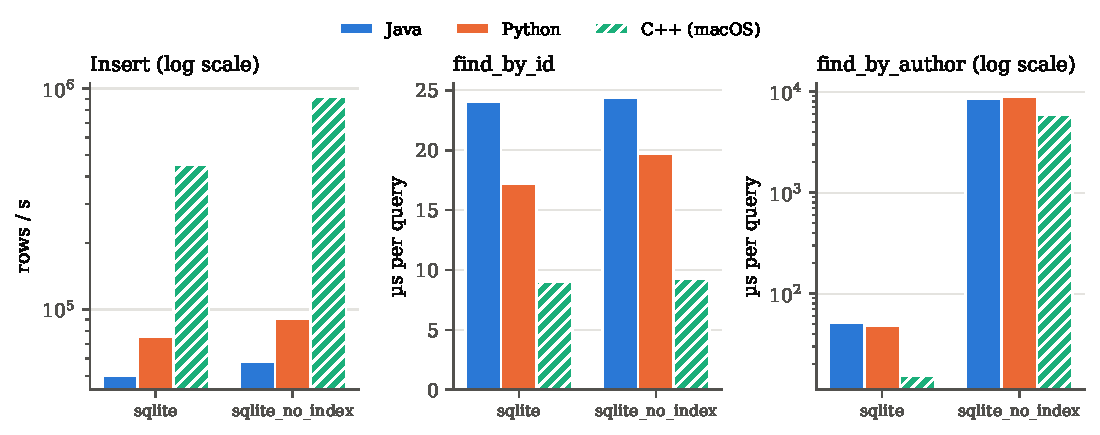
\includegraphics[width=\linewidth]{figures/lang_metadata.pdf}
\caption{Metadata with 100,000 generated rows, median of 5 runs. Hatched: C++, measured on macOS.}
\end{figure}

\begin{table}[H]
\centering\small
\begin{tabular}{@{}llrrr@{}}
\toprule
Metric ($N = 100{,}000$) & Variant & Java & Python & C++\,$^\dagger$ \\
\midrule
Insert (rows/s) & \code{sqlite} & 50,036 & 75,256 & \win 454,570 \\
 & \code{sqlite\_no\_index} & 58,103 & 90,399 & \win 915,179 \\
\code{find\_by\_id} (\us) & \code{sqlite} & 24.0 & 17.2 & \win 9.0 \\
\code{find\_by\_author} (\us) & \code{sqlite} & 52.0 & 48.8 & \win 15.4 \\
 & \code{sqlite\_no\_index} & 8,460 & 8,834 & \win 5,869 \\
\bottomrule
\end{tabular}
\caption{Metadata. $^\dagger$~measured on macOS.}
\end{table}

\begin{itemize}
  \item \textbf{The conclusion about the structure is the same in the three languages}: without the
        \code{author} index a lookup is a full scan that grows with the table, 160--380 times slower
        at 100,000 rows; with it, lookups stay flat.
  \item \textbf{Between Java and Python (same machine), Python is faster here}: SQLite is C code in
        both, and \code{executemany} in the \code{sqlite3} module hands a whole batch to C code,
        while JDBC adds the cost of its binding layer to every row. Python inserts 1.5 times faster;
        queries by author are equal within 10\%.
  \item \textbf{C++ calls the SQLite C API directly}, with no binding layer, and is 3--9 times faster.
        Part of this gap is the different machine and disk, so it cannot be read as a pure language
        result; the \code{sqlite\_no\_index} scans, which are pure SQLite work, show the machine
        effect alone at about 1.5 times.
\end{itemize}

\subsection{Overall view}
\begin{figure}[H]
\centering
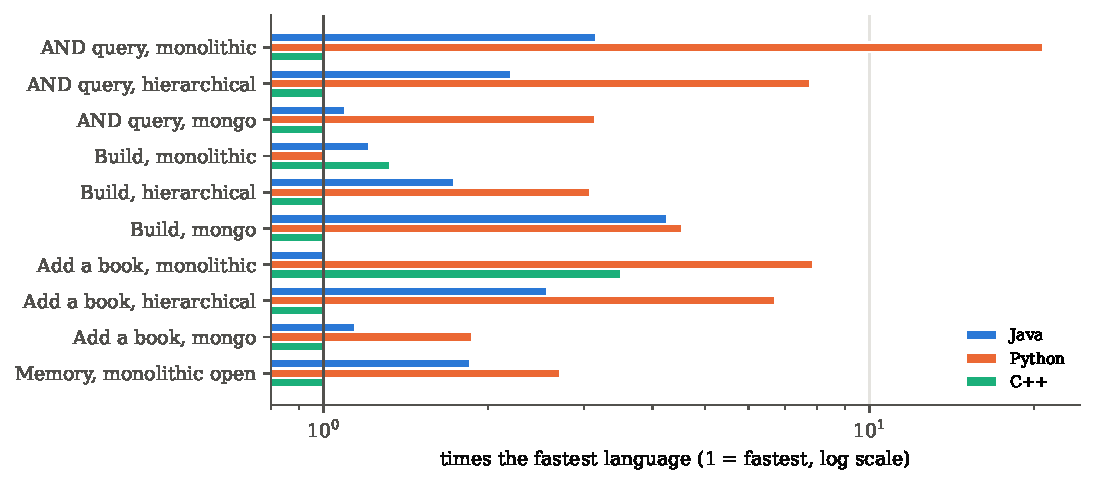
\includegraphics[width=\linewidth]{figures/lang_ratios.pdf}
\caption{Cost of each language relative to the fastest one ($= 1$) in the index experiments, $N = 200$,
all measured on the same Linux machine.}
\label{fig:ratios}
\end{figure}

\begin{table}[H]
\centering\small
\begin{tabularx}{\linewidth}{@{}L{4.3cm} Y L{2.6cm}@{}}
\toprule
Where the time goes & What the measurements show & Ranking \\
\midrule
In the program's own loops (queries, intersections, per-term work) & C++ fastest; Java 1.1--3.2 times; Python 3--21 times & C++ $>$ Java $\gg$ Python \\
In the operating system (writing large files) & Within 20\%; Python slightly ahead & All equal \\
Many small system calls (lookups, 129,356 files) & Interpreter overhead per call: Python 3--8 times Java & C++ $>$ Java $>$ Python \\
In C libraries (JSON, SQLite) & Depends on the binding: Python's C modules beat JDBC; Jackson beats nlohmann/json & Mixed \\
In an external server (MongoDB) & Round trips dominate; Java within 15\% of C++ & C++ $\approx$ Java $>$ Python \\
Memory of in-memory structures & 1 : 1.9 : 2.7 (C++ : Java : Python) & C++ $>$ Java $>$ Python \\
\bottomrule
\end{tabularx}
\caption{Where the differences between languages come from.}
\label{tab:where}
\end{table}

Figure~\ref{fig:ratios} and Table~\ref{tab:where} summarise the comparison. \textbf{C++} is the
fastest in 7 of the 9 time-based index experiments and uses the least memory. \textbf{Java} wins the
\code{monolithic} update and is the second fastest in the other eight; its gap with C++ is at most
3.2 times on queries and 4.3 times overall, the latter in the \code{mongo} build, which is a design
difference. \textbf{Python} is competitive only where the work is
delegated to C code or to the operating system; in its own loops it is the slowest by a wide margin.

% ================================================================ 7
\section{Choosing the language for the project}\label{sec:choice}

\subsection{What the project needs}
The language chosen now will carry the search engine into the next stages, where the data layer
grows (more books, continuous ingestion) and is used by services (indexing and query processes
running at the same time, likely distributed). From Stage~1 the requirements are:
\begin{enumerate}
  \item \textbf{Low query latency}, since queries are what users wait for.
  \item \textbf{Indexing and ingestion throughput}, to keep up with a growing collection.
  \item \textbf{Reasonable memory per posting}, while the index lives in memory.
  \item \textbf{Development effort and maintainability} for a team of three.
  \item \textbf{Portability and deployment} on the members' machines, the grader's machine and
        containers.
  \item \textbf{Ecosystem for the next stages}: database drivers, HTTP and service frameworks,
        distributed processing.
  \item \textbf{Safety of a shared codebase}: catching errors at compile time, no memory corruption.
\end{enumerate}

\subsection{How each language meets them}
\begin{table}[H]
\centering\small
\begin{tabularx}{\linewidth}{@{}L{2.9cm} c Y Y Y@{}}
\toprule
Criterion & Weight & Java & Python & C++ \\
\midrule
Query latency & 20 & \textbf{2} --- 1.1--3.2$\times$ C++ & \textbf{1} --- 3--21$\times$ C++ & \textbf{3} --- fastest everywhere \\
Indexing throughput & 20 & \textbf{2} --- best \code{monolithic} update, 2nd elsewhere & \textbf{1} --- slowest except \code{monolithic} build & \textbf{3} --- fastest in 4 of 6 \\
Memory & 10 & \textbf{2} --- 1.9$\times$ C++ & \textbf{1} --- 2.7$\times$ C++ & \textbf{3} --- least \\
Development effort & 15 & \textbf{2} --- 4,800 lines, verbose but plain & \textbf{3} --- 2,900 lines, the shortest & \textbf{1} --- 5,200 lines, manual resource handling \\
Portability, deployment & 10 & \textbf{3} --- JDK + Maven fetch everything & \textbf{3} --- \code{pip install} & \textbf{1} --- toolchain and native drivers per platform \\
Ecosystem for next stages & 15 & \textbf{3} --- JVM big-data and service stack & \textbf{2} --- strong for data analysis & \textbf{1} --- fewest ready-made pieces \\
Safety of shared code & 10 & \textbf{3} --- static types, memory safe & \textbf{1} --- dynamic types & \textbf{2} --- static types, not memory safe \\
\midrule
\textbf{Weighted score} (of 3) & 100 & \textbf{2.35} & \textbf{1.65} & \textbf{2.10} \\
\bottomrule
\end{tabularx}
\caption{Decision matrix. Scores: 3 best, 1 worst, from the measurements of Section~\ref{sec:times}
and the experience of building the three implementations.}
\label{tab:matrix}
\end{table}

Some notes on the scores:
\begin{itemize}
  \item \textbf{Performance (criteria 1--3)} comes from the index experiments, the only ones measured on
        the same machine for the three languages.
  \item \textbf{Deployment} was a real issue during Stage~1: the C++ module needs a C++20 compiler,
        CMake, Ninja, SQLite, libcurl and mongo-cxx-driver~4.x, which on Linux has to be built from its sources,
        while Java needs only a JDK and Maven, and Python only \code{pip}. A C++ test also failed only on
        Linux and had to be reproduced in a container.
  \item \textbf{Ecosystem.} The official MongoDB, SQLite and HTTP clients exist for the three, but the
        tools typically used to scale a data system across machines (distributed caches, message
        queues, Hadoop and Spark, mature web frameworks) are native to the JVM, available from Python,
        and rarely first-class in C++.
  \item \textbf{Sensitivity.} With the three performance criteria weighted at 50\%, Java wins. C++
        only overtakes Java if performance weighs more than 60\% of the decision. Python scores at
        least as low as Java on every performance criterion and does not beat it on the rest, so no
        weighting makes it the first choice for the core system.
\end{itemize}

\subsection{Recommendation}
\begin{note}
\textbf{The group recommends Java as the main language of the project.} It is the best balance
between the measured performance and the needs of a system that will grow and be developed by a
team: within 1.1--3.2 times of C++ on every query, second only to C++ in the other index
experiments, and the fastest at updating the selected \code{monolithic} index; 2--21 times faster than Python where the program's own code runs;
the simplest to deploy and to test (357 tests, contract tests over every structure); and the
language with the strongest ecosystem for the distributed stages to come.
\end{note}

The other two implementations keep a role:
\begin{itemize}
  \item \textbf{C++} is the choice if a later stage needs a single, latency-critical query service on a
        memory-constrained node: it answers \code{monolithic} queries 3.2 times faster than Java and
        holds the index in half the memory. Its cost is development time, portability and the lack of
        atomic writes in the current module.
  \item \textbf{Python} is the choice for everything around the system: analysis of results, the
        report charts, quick prototypes and data exploration. Its benchmarks show it is competitive
        when the heavy work runs in C (SQLite, JSON) or in the operating system, but its interpreted
        per-term loops make it the wrong choice for the indexing and query core.
\end{itemize}

% ================================================================ 8
\section{Conclusions and future improvements}

\subsection{Conclusions}
\begin{itemize}
  \item The group delivered the Stage~1 data layer three times, in Java, Python and C++, with the
        same contract, the same outputs byte for byte, and the same 12 benchmark experiments in a
        common CSV format.
  \item The structures to use do not depend on the language: \code{book}, \code{monolithic} and
        SQLite with indexes win in the three, and the three show the same limits (\code{monolithic}'s
        growing update cost and memory, \code{hierarchical}'s 73-fold block overhead, \code{time}'s
        slow lookups).
  \item The language matters in proportion to how much of the time is spent in the program's own
        code: up to 21 times for in-memory queries, about 1.1 times when a server or the file system
        does the work. C++ is the fastest, Java close behind, Python several times slower in its own
        loops.
  \item Some of the largest gaps come from design rather than language (C++'s \code{insert\_many}
        build and in-memory \code{time} lookup; the serialiser behind each \code{monolithic} update).
        Comparing implementations of the same contract makes these visible.
  \item Weighing performance with development, deployment, safety and ecosystem, \textbf{Java} is the
        language that best fits the project.
\end{itemize}

\subsection{Limitations and future improvements}\label{sec:future}
\begin{itemize}
  \item \textbf{One machine for everything.} The C++ datalake and metadata experiments should be rerun
        on the Linux machine used for the rest, to remove the hardware factor from those comparisons.
  \item \textbf{Larger collections.} At 200 books the \code{monolithic} index still wins; the point at
        which another structure takes over (extrapolated at roughly 700 books in C++, where
        \code{hierarchical} becomes cheaper to update, and 2,000--2,500 in Java, where \code{mongo}
        does) depends on the language and should be measured with thousands of books.
  \item \textbf{Aligning the designs that are not language-bound}: the same Mongo build strategy, a
        \code{time} lookup that survives a restart, and grouped flushes in Python, so that the
        remaining differences are only the languages'.
  \item \textbf{Other metadata backends.} The optional comparison of SQLite with a client--server
        relational database (PostgreSQL) and a NoSQL store (MongoDB) would show the cost of
        concurrent access, which Stage~2 will need.
  \item \textbf{Concurrency.} Stage~1 is single-threaded in the three languages; the next stages will
        need parallel tokenization and concurrent queries, where the languages differ again (threads
        in Java and C++, processes in Python because of the global interpreter lock).
\end{itemize}

% ================================================================ appendix
\appendix
\section{Repository and reproduction}
\subsection{Repository}
The source code is hosted at \url{https://github.com/BigData-Ulpgc/stage_1}, following the
\code{https://github.com/<group\_name>/stage\_1} format. It contains:
\begin{itemize}
  \item a \code{README.md} with the architecture, the requirements of each language, and the commands
        to build, test, run the pipeline and run the benchmarks of each implementation;
  \item \code{shared/}: the common contract (\code{SPEC.md}), the 200 book ids, the stopwords and the
        query workload;
  \item \code{sample\_dataset/}: the first 15 books, raw (\code{raw/pg<ID>.txt}, the pipeline input)
        and already split (\code{book/<ID>/}, the expected output), so instructors can test the
        pipeline without network;
  \item \code{java/stage1/}, \code{python/stage\_1/} and \code{cpp/}: the three implementations, each
        with its own guide, technical report and committed benchmark results;
  \item \code{docs/}: this report and its sources;
  \item a Git history of more than 150 commits between 17 September and 4 October 2026 that shows how
        the three implementations progressed.
\end{itemize}

\subsection{Quick test with the sample dataset}
Without network, each implementation runs the pipeline on the 15 sample books and answers the same
query with books 76, 84 and 2701:
\begin{lstlisting}
java -cp "$CP" es.ulpgc.bigdata.Main pipeline 30 --offline        # java/stage1/
python -m src.main.bigdata.main pipeline 15 --offline-source ../../sample_dataset/raw   # python/stage_1/
./build/release/search_engine_stage1 pipeline 30 --offline         # cpp/
... search whale island
\end{lstlisting}

\subsection{Reproducing the benchmarks}
From the repository root, \code{docker compose up -d} starts the group's MongoDB (optional: without
it, the \code{mongo} structure is skipped with a warning).

\textbf{Java} (from \code{java/stage1/}):
\begin{lstlisting}
mvn package
mvn -q dependency:build-classpath -Dmdep.outputFile=target/classpath.txt
CP="target/classes:$(cat target/classpath.txt)"
java -cp "$CP" es.ulpgc.bigdata.Main pipeline 400
java -cp "$CP" es.ulpgc.bigdata.benchmark.DatalakeBenchmark data/datalake/book
java -cp "$CP" es.ulpgc.bigdata.benchmark.IndexBenchmark 50,100,200 data/datalake/book
java -cp "$CP" es.ulpgc.bigdata.benchmark.MetadataBenchmark 1000,10000,100000
\end{lstlisting}

\textbf{Python} (from \code{python/stage\_1/}):
\begin{lstlisting}
pip install -r ../requirements.txt pytest
python -m src.main.bigdata.main pipeline 200
python -m src.main.bigdata.benchmark.benchmark_runner data/datalake/book
python -m src.main.bigdata.benchmark.benchmark_runner
python -m src.main.bigdata.benchmark.verify_results
\end{lstlisting}

\textbf{C++} (from \code{cpp/}):
\begin{lstlisting}
make && make test
B=./build/release/search_engine_stage1
$B pipeline 400
$B benchmark datalake_write      # one call per experiment, 12 in total
$B benchmark index_build
$B benchmark metadata_query
\end{lstlisting}

\textbf{This report} (from \code{docs/report/}): \code{uv run --with matplotlib python charts.py}
reads the committed CSVs of the three languages and draws the figures; \code{pdflatex report.tex}
twice builds the PDF.

\end{document}
